\fontsize{13px}{13px}\selectfont\justifying

\clearpage
\subsection{Sơ đồ lớp}
\FloatBarrier
\begin{figure}[!htbp]\fontsize{13px}{13px}\selectfont
	\centering
	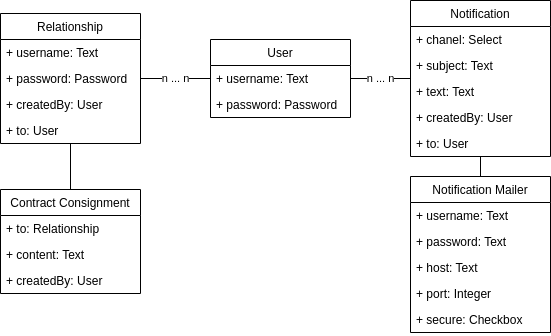
\includegraphics[width=0.8\textwidth]{class-accounts}
	\caption{Sơ đồ lớp quản lý kết bạn và chia sẻ}
	\justifying
	Các lớp thực hiện chức năng đăng nhập, đăng xuất, đăng ký. Gửi lời mời kết bạn, đồng ý kết bạn. Gửi yêu cầu chia sẻ sản phẩm. Thực hiện các chức năng thông báo.
\end{figure}

\FloatBarrier
\begin{figure}[!htbp]\fontsize{13px}{13px}\selectfont
	\centering
	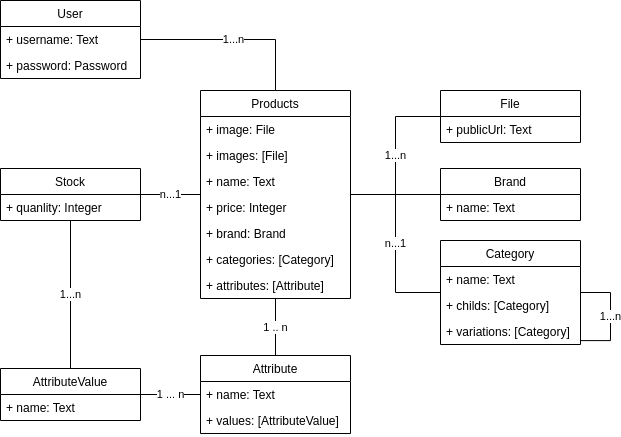
\includegraphics[width=0.8\textwidth]{class-products}
	\caption{Sơ đồ lớp quản lý sản phẩm}
	\justifying
	Các lớp thực hiện chức năng quản lý sản phẩm và tồn kho. Sản phẩm có nhiều thuộc tính và nhóm thuộc tính như màu sắc và kích thước. Đối với từng tổ hợp nhóm thuộc tính sẽ có một số lượng kho tương ứng.
\end{figure}

\clearpage
\FloatBarrier
\begin{figure}[!htbp]\fontsize{13px}{13px}\selectfont
	\centering
	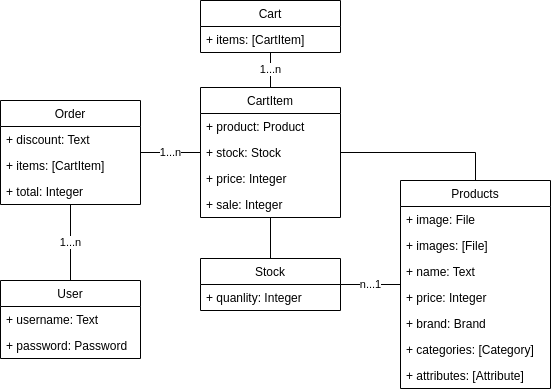
\includegraphics[width=0.8\textwidth]{class-orders}
	\caption{Sơ đồ lớp đặt hàng, quản lý đơn hàng}
\end{figure}
\FloatBarrier
\begin{figure}[!htbp]\fontsize{13px}{13px}\selectfont
	\centering
	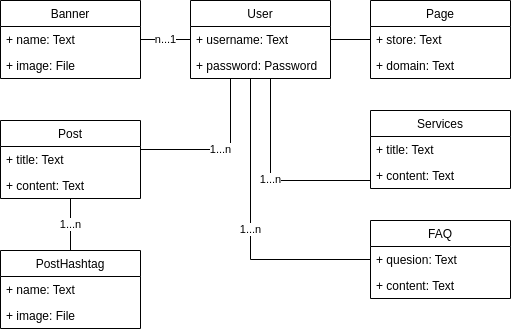
\includegraphics[width=0.8\textwidth]{class-store}
	\caption{Sơ đồ lớp quản lý cửa hàng}
\end{figure}